\documentclass[11pt]{article}

\usepackage[T1]{fontenc}
\usepackage{lmodern}
\usepackage[margin=1in]{geometry}
\usepackage{amsmath,amssymb}
\usepackage{graphicx}
\usepackage{booktabs}
\usepackage{tabularx}
\usepackage{array}
\usepackage{enumitem}
\usepackage{xcolor}
\usepackage{tikz}
\usetikzlibrary{positioning,arrows.meta}
\usepackage[numbers,sort&compress]{natbib}
\usepackage[hidelinks]{hyperref}
\usepackage{microtype}
\usepackage[section]{placeins}   % keep floats inside their own section

\setlist{itemsep=2pt,topsep=4pt}
\newcolumntype{L}{>{\raggedright\arraybackslash}X}
% \gl{term}: first use of a term defined in the glossary (Appendix A); prints a dagger linked to it
\newcommand{\gl}[1]{#1\hyperref[app:glossary]{$^{\dagger}$}}

\title{How an AI Economy Behaves: A Multi-Agent Simulation in Which AI Companies Learn to Compete by Reinforcement Learning}
% Author line: the aiXiv version (default) lists Claude Code as author; the arXiv bundle sets \aixivfalse,
% because arXiv does not accept AI tools as authors.
\newif\ifaixiv \aixivtrue
\ifaixiv
\author{Claude Code (Anthropic)\\[2pt]with inspiration from Ravi Kadam\\Independent Researcher (corresponding human)\\\texttt{ravindrakad@gmail.com}}
\else
\author{Ravi Kadam\\Independent Researcher\\\texttt{ravindrakad@gmail.com}}
\fi
\date{October 2026}

\begin{document}
\maketitle

\begin{abstract}
We present an open, reproducible simulation of a stylised AI industry over ten years in which AI product companies learn to compete by reinforcement learning (RL). It links a chip fabricator, chip designers, data centres, frontier and open-weight model providers, 5--12 AI product companies and 300 enterprise customers in three sectors; companies choose use cases, models, budgets and when to pilot, launch, scale or stop, facing uncertain technology, hidden customer value, compute shortages and rivals. With the test plan fixed in advance, five PPO agents trained on a laptop created \$19.3M of value per company on 100 unseen markets against \$14.3M for the strongest hand-written rule; four of five were clearly better, narrowly missing our pre-set bar of five. They also led under faster or slower technology progress and a wave of entrants, but showed no detectable difference from the rule in a severe compute crunch, where they went bankrupt more often. RL added \$4.7M over imitating the rule; learning from scratch succeeded in three of five runs, and its successes outperformed imitation-started agents. We also introduce Paired-Fork Advantage against a Rule (PFAR), which copies the market mid-game and compares the agent's action with the rule's under identical future randomness. PFAR cut the noise of the learning signal 1.7--3.9 fold but, in a pre-registered test, produced no better agents. In the simulated market, adoption follows S-curves, the regulated sector is held back by reliability, first launchers gain no lasting share, and supply shocks nearly quadruple compute prices. Written for readers new to RL, with a glossary. Code, agents and a live viewer are open source.
\end{abstract}

\section{Introduction}

The AI industry is a chain of businesses that depend on one another, and the chain behaves in ways no single company controls. Chip factories decide how much capacity to build years ahead. Data centres buy those chips and rent out computing power. Model labs sell access to AI models. Product companies build AI applications on those models, and enterprises decide whether the applications are worth paying for. A shortage, a breakthrough or a wave of failed projects at any point ripples through all the others.

These ripples are hard to reason about and impossible to experiment with in reality. Nobody can rerun the last five years with one chip factory fewer, or with model progress twice as fast. A simulation can: it lets us build a small, transparent version of the industry, change one assumption at a time, and watch what follows.

This paper describes such a simulation, the \emph{AI Economy Lab}, and uses it for two purposes:
\begin{enumerate}
  \item \textbf{To understand market dynamics.} How does enterprise adoption spread? What does a supply shock do to prices, failures and competition? Does being first to market pay?
  \item \textbf{To study decision-making under uncertainty.} We let software agents learn, by trial and error, how to run an AI product company in this market, using reinforcement learning. We then ask what strategies they discover, whether they beat sensible hand-written rules, and whether that result holds up on markets they have never seen.
\end{enumerate}

No background in reinforcement learning or economics is assumed. Terms marked with a dagger ($^\dagger$) are explained in plain words where they first appear and collected in a glossary (Appendix~\ref{app:glossary}). Sections~\ref{sec:scenario} and~\ref{sec:rules} describe the scenario and its rules, Section~\ref{sec:competitors} introduces the competitors, and Section~\ref{sec:results} presents the results, explaining each reinforcement-learning idea where it matters. Section~\ref{sec:lessons} separates what the simulation shows from what it might imply for real markets.

Our contributions are: (i) an open simulator of a multi-layer AI value chain with audited accounting and fifteen automated checks; (ii) a training recipe that runs on a laptop, with every change, test market and success criterion written down before the v2 experiments; (iii) a test of five independently trained agents and three five-run comparison arms on 350 test markets across six market conditions, plus a yardstick check and sensitivity analysis on fresh markets, reported in full including where the agents fall short; (iv) \emph{Paired-Fork Advantage against a Rule} (PFAR), a policy-gradient advantage estimator for simulators that can be copied mid-episode: it compares the agent's action with an expert rule's action in two copies of the market that share all future randomness, giving a valid-baseline signal for delayed decisions whose noise is 1.7--3.9 times lower; under a pre-registered test it did not produce better agents than plain PPO, and its benefit for learning from scratch was at most suggestive; and (v) an educational treatment that ties each reinforcement-learning idea to a result the reader can see. The reinforcement-learning machinery other than PFAR is standard. Every parameter is an illustrative assumption chosen to be plausible, not a measurement of the real industry; the value of the exercise lies in the mechanisms it makes visible.

\section{Related work}
\label{sec:related}

\textbf{Agent-based economics.} Agent-based computational economics studies markets as systems of interacting, boundedly rational agents rather than as equilibria \citep{tesfatsion2006ace,farmer2009economy}. Our simulator follows this tradition with a stylised multi-layer value chain, adding learning agents to one layer.

\textbf{Reinforcement learning in economic settings.} The AI Economist used two-level multi-agent RL to design tax policy in a simulated economy \citep{zheng2022aieconomist}, and RL pricing agents have been shown to learn collusive behaviour \citep{calvano2020collusion}. We focus instead on company strategy in a technology market with stage-gated projects, uncertain feasibility and supply-chain delays.

\textbf{Multi-agent RL market simulators.} Closest in spirit are simulators built for learning agents in markets. ABIDES simulates a stock exchange with tens of thousands of agents \citep{byrd2019abides}; ABIDES-Gym wraps it for single learning agents \citep{amrouni2021abidesgym}, and ABIDES-MARL adds several learning agents that trade in a limit order book with endogenous liquidity \citep{cheridito2025abidesmarl}. Multi-agent RL bidders in electricity markets can learn tacitly collusive prices \citep{seredynski2026electricity}. These study trading or bidding against prices set seconds to days ahead. Our setting differs in what is decided and how slowly it pays off: companies commit to multi-month projects behind technical and commercial gates, on top of a supply chain with build-out lags of years, so a decision's consequences arrive 8--12 months later. That long, gated credit assignment is what motivates the method in Section~\ref{sec:pfar}.

\textbf{Counterfactual rollouts and common random numbers.} Fixing a simulator's randomness to compare policies goes back to PEGASUS \citep{ng2000pegasus}, and branching rollouts from a shared state appear in the ``vine'' variant of TRPO \citep{schulman2015trpo}. Counterfactual baselines for multi-agent credit assignment are usually learned critics \citep{foerster2018coma}. Recent work forks restorable environments to give software-engineering agents a per-step signal \citep{li2026crr}, pairs LLM-agent rollouts under shared noise and shows that this does not always reduce gradient variance \citep{sakib2026luck}, and uses common random numbers for planning with rollouts \citep{yadav2026crn}. Our method differs from these in using an expert rule's action as the counterfactual, which makes the comparison a valid baseline, and in sharing every random stream of a multi-agent market.

\textbf{Methods.} We use Proximal Policy Optimisation \citep{schulman2017ppo} with generalised advantage estimation \citep{schulman2016gae}; PPO with one network shared by many agents is a strong baseline in multi-agent settings \citep{yu2022mappo}. Starting RL from imitation of an expert goes back to ALVINN \citep{pomerleau1991alvinn} and was central to AlphaGo \citep{silver2016alphago}; the weaknesses of pure imitation are analysed by \citet{ross2011dagger}. Training against frozen past versions of oneself steadies multi-agent learning \citep{vinyals2019alphastar}. Our treatment of project spending follows potential-based reward shaping \citep{ng1999shaping}, and we remove impossible actions before the agent chooses \citep{huang2022masking}. Standard texts cover the foundations \citep{sutton2018rl}.

\textbf{Generalisation and evaluation.} RL agents can overfit to the situations they trained on \citep{cobbe2019generalization}; training on randomised conditions is a common remedy \citep{tobin2017domain}. Results in deep RL vary greatly between training runs and need many independent runs and honest uncertainty estimates \citep{henderson2018matters,agarwal2021precipice}. We follow that advice and also fix our test plan in advance.

\textbf{Market dynamics.} Our supply chain shows the delayed, amplified responses familiar from the bullwhip effect \citep{lee1997bullwhip} and from experiments on misread feedback \citep{sterman1989misperceptions}. Adoption follows the S-shaped diffusion described by \citet{bass1969diffusion} and \citet{rogers2003diffusion}. We test first-mover advantage \citep{lieberman1988firstmover} in a market where all companies share the same underlying models. Business simulation games have long been used in management education \citep{faria2009gaming}; our live viewer serves a similar purpose.

\section{The scenario}
\label{sec:scenario}

The simulation follows a stylised AI industry for ten years, one month at a time. Six kinds of players form a supply chain (Figure~\ref{fig:valuechain}). Only one kind, the AI product companies, makes the strategic choices this study is about; the others follow fixed rules designed to behave like their real counterparts.

\begin{figure}[t]
\centering
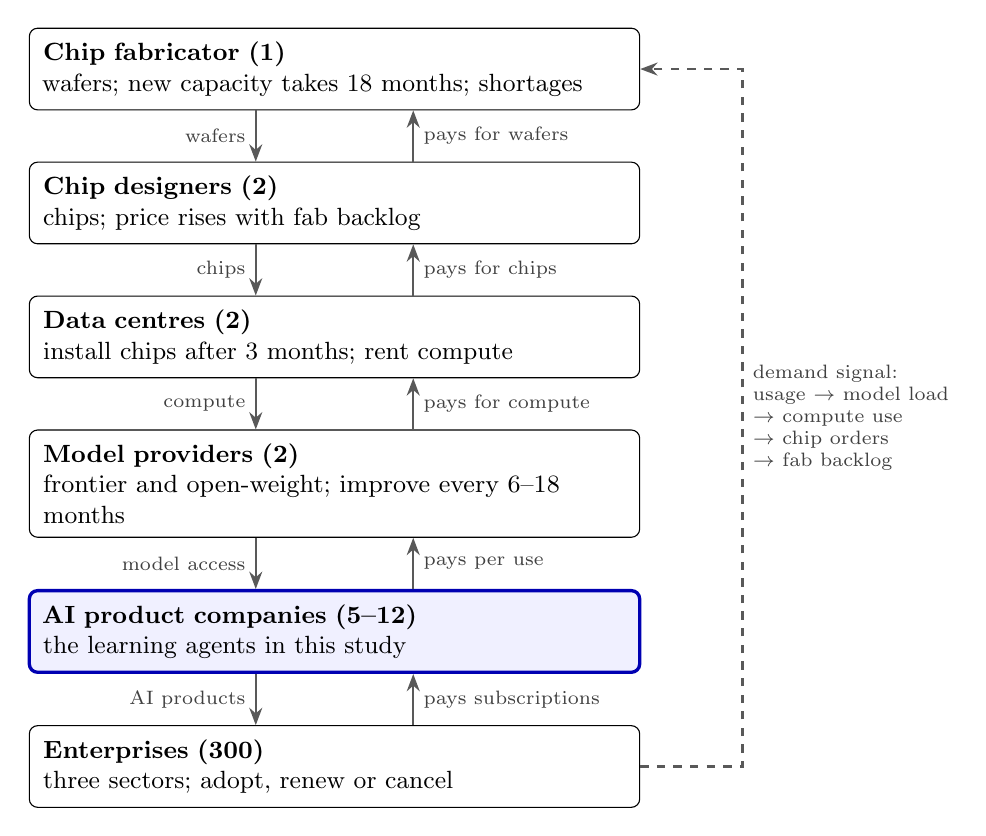
\begin{tikzpicture}[
  box/.style={draw, rounded corners=3pt, text width=7.4cm, minimum height=1.0cm, align=left, font=\small, inner sep=5pt},
  hl/.style={box, draw=blue!70!black, fill=blue!6, very thick},
  arr/.style={-{Stealth[length=2.2mm]}, thick, gray!70!black},
  lab/.style={font=\scriptsize, text=gray!50!black}]
\node[box] (fab) {\textbf{Chip fabricator (1)}\\ wafers; new capacity takes 18 months; shortages};
\node[box, below=0.65cm of fab] (chip) {\textbf{Chip designers (2)}\\ chips; price rises with fab backlog};
\node[box, below=0.65cm of chip] (dc) {\textbf{Data centres (2)}\\ install chips after 3 months; rent compute};
\node[box, below=0.65cm of dc] (mod) {\textbf{Model providers (2)}\\ frontier and open-weight; improve every 6--18 months};
\node[hl, below=0.65cm of mod] (bld) {\textbf{AI product companies (5--12)}\\ the learning agents in this study};
\node[box, below=0.65cm of bld] (ent) {\textbf{Enterprises (300)}\\ three sectors; adopt, renew or cancel};
\foreach \a/\b/\p/\m in {fab/chip/wafers/pays for wafers, chip/dc/chips/pays for chips, dc/mod/compute/pays for compute, mod/bld/model access/pays per use, bld/ent/AI products/pays subscriptions} {
  \draw[arr] ([xshift=-1.0cm]\a.south) -- node[left, lab] {\p} ([xshift=-1.0cm]\b.north);
  \draw[arr] ([xshift=1.0cm]\b.north) -- node[right, lab] {\m} ([xshift=1.0cm]\a.south);
}
\draw[arr, dashed] (ent.east) -- ++(1.3,0) |- node[pos=0.25, right, lab, align=left] {demand signal:\\usage $\rightarrow$ model load\\$\rightarrow$ compute use\\$\rightarrow$ chip orders\\$\rightarrow$ fab backlog} (fab.east);
\end{tikzpicture}
\caption{The simulated AI industry. Goods flow down the chain; money and the demand signal flow back up, each with its own delays.}
\label{fig:valuechain}
\end{figure}

\textbf{Upstream suppliers.} One fabricator produces wafers; two chip designers turn them into chips of different efficiency and price; two data centres buy the chips and sell computing power in GPU-equivalent units. A data centre orders chips after it has been more than 80\% busy; chips arrive months later; a new fab line takes 18 months. From time to time the fab loses 30--60\% of its output for 3--9 months.

\textbf{Model providers.} A \emph{frontier} model is more capable and more reliable but expensive; an \emph{open-weight} model is cheaper but weaker. Both improve at random intervals of 6--18 months, occasionally in a large jump, and the open model closes part of the gap at each release. Capability is tracked separately for each customer sector.

\textbf{AI product companies.} Each starts with \$1.5M in cash and a \$400k credit line, can run at most three projects, and has a skill level and a risk appetite (cautious, balanced or aggressive). New companies enter from month 12 when incumbents are profitable, up to 12 in the market; companies that cannot pay their bills go bankrupt.

\textbf{Enterprises.} Three hundred enterprises in three sectors that value different things (Table~\ref{tab:sectors}). Each enterprise has a \emph{confidence} in AI products (0--1) that rises with successful pilots, falls with failures and cancellations, and spreads within its sector.

\begin{table}[h]
\centering
\small\setlength{\tabcolsep}{4pt}
\begin{tabular}{lrrlll}
\toprule
Sector & Firms & AI budget & Values most & Reliability needed & Confidence \\
\midrule
Customer operations & 110 & \$40k/month & price & 70\% & 0.55 \\
Software engineering & 100 & \$60k/month & capability & 70\% & 0.60 \\
Regulated industries & 90 & \$80k/month & reliability & 84\% + per use case & 0.40 \\
\bottomrule
\end{tabular}
\caption{Enterprise sectors.}
\label{tab:sectors}
\end{table}

\textbf{Use cases.} The market contains 60 use cases: specific jobs AI could do for one sector. Twenty-four are visible at the start and the rest are discovered over time, faster once models can tackle them. Each has a hidden difficulty, a value per customer that companies see only as a noisy estimate, a number of enterprises that need it (8--35\% of the sector), a development time of 2--5 months per stage, an integration burden, an optional extra reliability requirement and a compute footprint per customer.

\textbf{An illustrative journey.} Suppose a software-engineering use case is worth \$18k a month to each of 30 enterprises. A company sees a difficulty estimate of 0.62 (true value 0.55, hidden). It starts a project on the frontier model with a standard budget (\$20k, then \$25k a month). After about three months of research and three of prototyping it faces the technical gate, with a success chance of about 82\%. It then pilots with three enterprises for two months and passes the commercial gate. It launches at about \$5.8k a month per customer; model usage costs about \$1.6k and support \$0.8k, leaving \$3.4k of margin. Limited to about three new customers a month, it reaches 20 customers and about \$68k monthly profit after seven months, until a rival competes or compute prices rise.

\section{The rules of the simulation}
\label{sec:rules}

\subsection{The monthly cycle}
Every month runs the same steps in the same order, so the same random seed and decisions reproduce exactly the same history: (1) random shocks and queued arrivals; (2) publication of prices, capacity and confidence with a one-month lag; (3) simultaneous decisions by all companies, which cannot see rivals' current choices; (4) budget checks and fair random allocation of contested pilot customers; (5) project progress and gate draws; (6) adoption, cancellation and compute service; (7) settlement of costs, interest and bankruptcy; (8) price, confidence, supplier and entry updates; (9) scoring.

\subsection{Two kinds of uncertainty}
The \textbf{technical gate} asks whether the AI can do the job. Its success probability is
\begin{equation}
p = \mathrm{clip}_{[0.03,\,0.97]}\;\sigma\!\big(6\,(c_{m,s} - d) + \text{skill} + \text{effort} - 1.5\,b + 0.4\big),
\end{equation}
where $c_{m,s}$ is the chosen model's capability in the sector, $d$ the hidden difficulty, $b$ the integration burden and $\sigma$ the logistic function, which turns any number into a probability between 0 and 1. For a typical company, a model 0.2 weaker than the task gives about 50\%, a matched model about 77\%, and a model 0.2 stronger about 92\%. Failed projects can be retried at extra cost, and each attempt sharpens the company's difficulty estimate.

The \textbf{commercial gate} follows a two-month paid pilot with up to three enterprises. It passes only if pilot customers received more value than they paid plus their required return, and the model met their reliability requirement. When a sector's confidence is low, enterprises may refuse to pilot at all; this \emph{deferral} is recorded separately from failure.

\subsection{Buying decisions, compute and supply}
Each month every enterprise with an unmet need and budget compares offers, weighing expected benefit (rising with capability and reliability) against price and integration cost, scaled by its confidence. It picks the best offer, and each extra competitor lowers list prices by 12\%. Contracts take 1--4 months to sign, and a company onboards about three customers a month (nine after a \$150k scale-up). Customers who receive less value than expected are much more likely to cancel, and visible cancellations lower sector confidence.

Every customer consumes compute. When demand exceeds installed capacity, all buyers receive the same reduced share; unserved usage is not billed and raises cancellations. The compute price moves with utilisation between \$3 and \$30 per unit. Data centres order chips above 80\% utilisation, with about four months to install; the fab invests when its backlog exceeds 1.2 months of output, with an 18-month lead time. In every market we ran, the backlog never reached that trigger, so the fab's capacity stayed fixed and its build time never came into play (Section~\ref{sec:robust}).

\subsection{Money, value and information}
All money moves through a double-entry ledger whose balances always sum to zero. Main company costs are overhead (\$25k/month), development per project (\$12k, \$25k or \$50k per month for lean, standard or premium budgets), starting (\$20k), piloting (\$40k), launching (\$30k), scaling (\$150k) and support (\$0.8k per customer per month), plus model usage. Credit costs 1.2\% a month.

A company's \textbf{value} is its cash minus debt, plus the present value of its live products' recent profit, plus a cautious book value for projects in development. Its monthly change is the company's score and, in Section~\ref{sec:results}, the learning agent's reward.

Companies observe their own state, noisy estimates of use-case difficulty and value, last month's model capability, reliability and prices, sector confidence, and rivals' launches. True difficulty, enterprise-specific benefit, rivals' private decisions, future shocks and gate draws are hidden. Fifteen automated checks confirm that the same seed gives the same history, that there is no revenue without demand, that technical failure persists even with unlimited compute, that there is no adoption without a product, that prices rise under scarcity, that capacity lead times are respected, that the ledger balances, that no hidden information leaks to companies, and that a bankrupt company keeps no project value.

\subsection{The model as a whole}
\label{sec:formal}

Formally, the simulation is a partially observable stochastic game with a changing set of players. Let $\mathcal{I}_t$ be the companies alive in month $t$. The state $s_t$ has five blocks (Table~\ref{tab:state}). Each month
\begin{equation}
s_{t+1} = F\big(s_t,\ (a_{i,t})_{i\in\mathcal{I}_t},\ \xi_t\big),
\end{equation}
where $F$ applies the nine steps of Section~\ref{sec:rules} in order and $\xi_t$ are draws from separate seeded random streams (shocks, gate outcomes, entry, customer choices), so a seed fixes everything except the companies' decisions. Company $i$ sees only $o_{i,t} = O_i(s_t, \xi_t)$: its own state plus lagged and noisy market data. Its value $V_{i,t}$ and its score $r_{i,t} = (V_{i,t}-V_{i,t-1})/\$1\text{M}$ are defined in Appendix~\ref{app:reward}. Rule-based companies act by fixed functions $a_{i,t} = \pi^{\text{rule}}(o_{i,t})$; learning companies share one network $\pi_\theta(a \mid o_{i,t}, \text{risk profile}_i)$. Suppliers, model providers and enterprises are part of $F$, not players. Companies interact only through the market: shared customers and prices, shared compute, and sector confidence.

\begin{table}[h]
\centering
\small
\begin{tabularx}{\linewidth}{lLl}
\toprule
State block & Contents & Changed by \\
\midrule
Supply & fab capacity, backlog and build pipeline; chip prices; data-centre capacity and pending installs; compute price & capacity rules, shocks \\
Models & capability per sector, reliability, usage price for frontier and open models & random releases \\
Use cases & hidden difficulty and value, enterprises in need, integration burden, discovered or not & discovery \\
Enterprises & budget, needs, subscriptions, sector confidence & buying rule, pilots, cancellations \\
Companies & cash, debt, projects (stage, progress, investment, model, budget, customers), skill, reputation, risk profile & actions, gates, settlement \\
\bottomrule
\end{tabularx}
\caption{The simulation's state.}
\label{tab:state}
\end{table}

\textbf{Limiting cases.} Three simple limits are built in and checked. Without competition (each use case claimable by one company) the market becomes a set of separate monopolies; we use it as a switch-off test (Section~\ref{sec:ablation}). Without technical failure every gate depends only on customers. With unlimited compute there are no shortages, yet technical failure remains (an automated check). We do not derive equilibria or stability results: the analysis is computational, and the learned policy is trained against a fixed mix of rules and copies of itself, not shown to be a best response to anything.

\section{The competitors}
\label{sec:competitors}

Each month every company takes one action: hold, start a project (choosing use case, model and budget), pilot, launch, scale, retry, pause or abandon. Five kinds of decision-maker compete (Table~\ref{tab:competitors}). All rule-based strategies share sensible habits: they pilot and launch ready projects, retry or abandon failures, close persistent loss-makers and scale profitable products.

\begin{table}[h]
\centering
\small
\begin{tabularx}{\linewidth}{lL}
\toprule
Strategy & How it decides \\
\midrule
Random & Any allowed action at random (a control). \\
Easy-first & Starts the use case that looks easiest, on the frontier model with a standard budget. \\
Best expected value & Scores every use case, model and budget by a hand-built estimate of success odds $\times$ profit and picks the best. This is the strongest rule and our main yardstick. \\
Cash-preserving & One project at a time, open model, lean budget, only with 12 months of cash in hand. \\
\textbf{Learning agent} & A neural network that improves by playing thousands of simulated markets (reinforcement learning). \\
\bottomrule
\end{tabularx}
\caption{The competing decision-makers.}
\label{tab:competitors}
\end{table}

The learning agent sees what a real company could: its finances and projects, a shortlist of 12 use cases with noisy estimates, and last month's market data (415 numbers in total). One network controls every learning company in a market, so it also learns from playing against copies of itself.

\section{Results, and the reinforcement learning behind them}
\label{sec:results}

\subsection{How an agent learns by trial and error}
\label{sec:learn}

\textbf{The basic loop.} Reinforcement learning trains an \gl{agent} (here, the decision-maker for one company) by letting it act in an \gl{environment} (the simulated market). Each month the agent receives an \gl{observation} of its situation, chooses an \gl{action}, and receives a \gl{reward}: the change in its company's value. Its goal is to maximise total reward over the ten-year game, called an \gl{episode}, not just the next month \citep{sutton2018rl}.

\textbf{The policy.} The agent's decision rule is its \gl{policy}: a neural network that turns an observation into a probability for each possible action. Training nudges the network so that actions followed by better-than-expected results become more likely. Repeated over millions of decisions, good behaviour can emerge without anyone writing it down.

\textbf{Why this is hard here.} Every investment looks like a loss for months. A project costs money at once; the payoff comes only after a correct chain of decisions (start, wait, pilot, wait, launch) 8--12 months later, and only if both gates pass. When a reward finally arrives, the agent must work out which earlier decisions deserve the credit, a difficulty known as the \gl{credit-assignment problem}. An agent that acts at random almost never completes the chain and mostly sees spending followed by lower value, so it is tempted to conclude that spending is bad. Organisations face the same trap when they judge a new kind of project by its first quarter's cash flow.

Three ingredients help the agent through this:
\begin{itemize}
  \item \textbf{A fairer score.} Money spent on projects still in development counts as a partly recoverable asset, written off if the project fails, is abandoned or the game ends. The undiscounted ten-year total of the score is unchanged, but investment no longer looks like an immediate loss. This is a form of \gl{reward shaping}, inspired by potential-based shaping \citep{ng1999shaping}. It is \emph{not} the exact form that guarantees an unchanged best strategy when future rewards are discounted, and the agent's training reward also adds deliberate penalties for losses, cash stress and bankruptcy, so the agent optimises a risk-adjusted goal rather than value alone. Appendix~\ref{app:reward} gives the exact equations.
  \item \textbf{Judging decisions against expectations.} Alongside the policy, the network learns a \gl{value function}: a prediction of how much future reward to expect from the current situation. Each action is then judged by its \gl{advantage}, how much better things turned out than predicted, which separates good decisions from good luck \citep{schulman2016gae}. Future rewards are discounted by 1\% a month, so a reward about six years away counts half as much as one today.
  \item \textbf{Small, safe steps.} We update the policy with \gl{Proximal Policy Optimisation} (PPO) \citep{schulman2017ppo}, which limits how far the policy may change in one update so that improvement stays steady.
\end{itemize}

\textbf{The reward in symbols.} The score is $r_t = (V_t - V_{t-1})/\$1\text{M}$, the monthly change in company value. The agent was trained on a risk-adjusted version,
\begin{equation}
\tilde r_t = r_t - \delta\max(0,-r_t) - c_t - 2\beta\,\mathbb{1}[\text{bankrupt at } t],
\end{equation}
discounted by 1\% a month, where $\delta$ is the company's aversion to losses (0.1--0.6 by risk appetite), $c_t$ a small charge when cash runway is short or debt is high, and $\beta$ its aversion to bankruptcy (0.7--3.0). So the agent was asked to create value while avoiding losses and bankruptcy, not to maximise value alone; Appendix~\ref{app:reward} gives every term.

\textbf{Exploration.} An agent that only repeats what has worked never discovers anything better, so it must keep trying alternatives. How much it varies its choices is called its \gl{exploration} level (technically, the entropy of the policy). Left alone, PPO tends to reduce exploration quickly as the agent grows confident, sometimes too quickly. We therefore set an \gl{exploration floor}: whenever the agent's exploration falls below a set level, its bonus for exploring rises automatically.

\textbf{Two ways to start.} An agent can start from random behaviour, or first copy an expert. Copying an expert's choices from recorded examples is called \gl{imitation learning} (also behaviour cloning) \citep{pomerleau1991alvinn}. We recorded about 115{,}000 decisions of the best-expected-value rule across 96 markets and trained the network to predict them; after six passes it matched the rule's choice of action type 98\% of the time. PPO then improves on this starting point. As a comparison, we also trained one agent from scratch, with no imitation.

\begin{figure}[h]
\centering
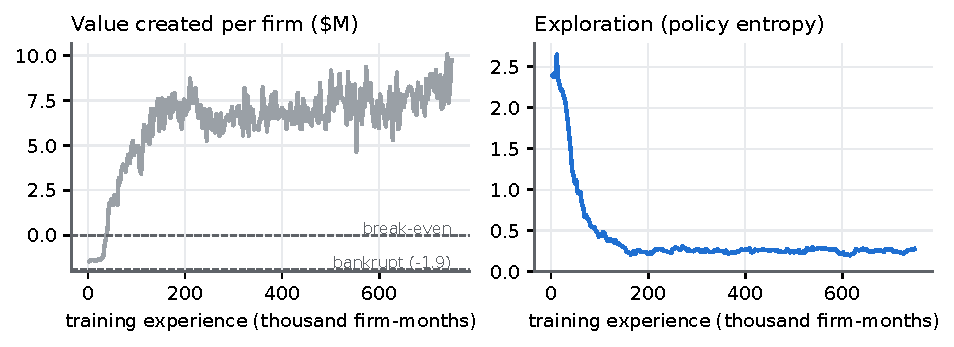
\includegraphics[width=\linewidth]{figures/fig_pure_rl.pdf}
\caption{Learning from scratch, with no imitation (one of the three successful runs out of five). Left: value created per company in the training games. Right: the agent's exploration level, which falls from 2.6 and then stays near the floor (0.25).}
\label{fig:purerl}
\end{figure}

Learning from scratch can work (Figure~\ref{fig:purerl}). In this run the agent lost money at first, crossed break-even within about 40{,}000 firm-months of experience, and kept improving while its exploration settled at the floor. It is not guaranteed: two of five such runs never escaped the do-nothing trap (Section~\ref{sec:controls}).

\textbf{Practical details.} An \gl{action mask} removes impossible choices (for example, launching a project that has not passed its pilot) before the agent chooses \citep{huang2022masking}. One network with shared parameters controls every learning company, with each company's risk appetite as an input \citep{yu2022mappo}. Training ran 24 markets at once across 6 CPU cores, in 60-month stretches. Rival seats in training markets were 50\% the learning agent itself, 35\% rule-based companies (including 5\% random) and 15\% frozen past versions of the agent \citep{vinyals2019alphastar}. The PPO update ran on the laptop's GPU and the many small per-month decisions on its CPU, which was faster for small batches.

\subsection{Avoiding overfitting: varied markets, practice markets and a test written down in advance}
\label{sec:protocol}

An agent can become very good at the exact markets it trained on and poor elsewhere, a problem called \gl{overfitting} \citep{cobbe2019generalization}. We guarded against it in three ways.

\textbf{Training on varied markets.} In 75\% of training games we drew a fresh set of market conditions: how often and how badly chip supply fails, data-centre capacity, build-out delays, how fast new rivals enter, how often and how far models improve, how hard use cases are, and how noisy companies' estimates are. This idea is called \gl{domain randomisation} \citep{tobin2017domain}. Every range stopped short of the five named test conditions described below, so those conditions remained genuinely new to the agent; a check in the code enforces this.

\textbf{Practice markets for choosing which version to keep.} Training produces a new version of the agent after every update, and some versions are better than others. Every 20 updates we scored the current version on 40 \gl{practice markets} (also called a validation or development set) that were never used for training or testing: 20 normal markets and 20 with varied conditions. We kept the best-scoring version and stopped after eight checks without improvement, a rule called \gl{early stopping}. Each version was scored in two modes, picking actions at random according to its probabilities (sampled) and always picking its most likely action (greedy), and the better mode was kept with it.

\textbf{A test plan fixed in advance.} Before the v2 experiments began we wrote down the training changes, the test markets, the measure of success and the bar for calling the result a success, a practice called \gl{pre-registration}. The plan was informed by an earlier, exploratory version of this study with the same simulator, whose results motivated the changes; no result from that version is used here. The test markets had never been used for anything: 100 normal markets and five changed conditions with 50 markets each (seeds 400--499 and 400--449). We ran the test once, after all training had finished, and report every result. The success bar was: all five agents clearly better than the strongest rule in normal markets, and an average lead of at least \$3M. Before any test result existed we added two comparison runs: three agents trained without varied markets, and one trained without imitation; after review both were extended to five runs (Appendix~\ref{app:audit}). Appendix~\ref{app:audit} lists what the record can and cannot prove about these dates, and every departure from the plan.

\textbf{Five training runs.} RL results can depend heavily on luck in training \citep{henderson2018matters}, so we trained five agents with the same recipe and different random seeds (each also used different training markets). Each took 13--30 minutes of computing on an Apple M2 Pro laptop and stopped early after 374{,}000--979{,}000 firm-months of experience.

\begin{figure}[h]
\centering
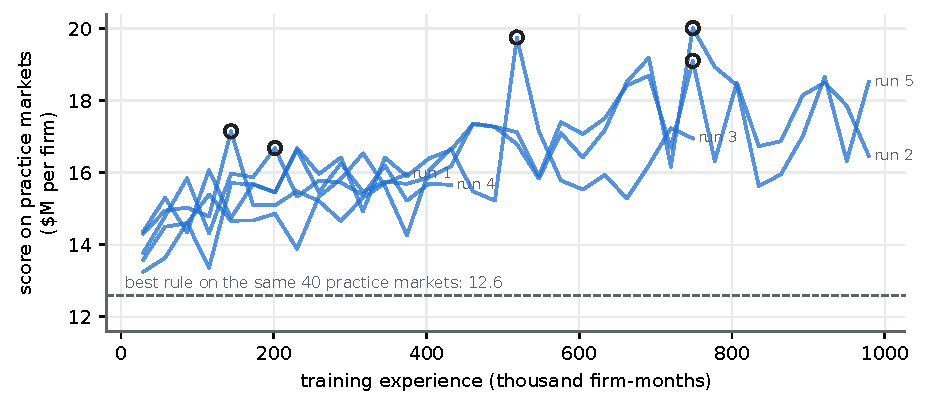
\includegraphics[width=\linewidth]{figures/fig_training.pdf}
\caption{Score on the 40 practice markets during training for each of the five runs. Circles mark the version kept. The dashed line is the best rule on the same markets.}
\label{fig:training}
\end{figure}

All five runs started near the rule's level and climbed above it (Figure~\ref{fig:training}). The curves zig-zag: a version's practice score moves by about \$2M from one check to the next partly through luck, and after a peak the policy often drifts lower. Early stopping keeps the peak version, but a peak chosen this way is partly lucky, which matters below.

\subsection{Does the learner beat the rules on markets it has never seen?}
\label{sec:test}

\textbf{A fair test.} In each test market one company's seat is played in turn by each candidate, while the other four companies and all new entrants follow the same fixed mix of rules. Because a market's randomness depends only on its seed, every candidate faces identical hidden difficulties, customer needs and shocks, so we can compare them market by market. In sampled mode each market's result is the average of three plays with different randomness; in greedy mode it is a single play.

\begin{table}[h]
\centering
\small\setlength{\tabcolsep}{4pt}
\begin{tabular}{lrrrr}
\toprule
Condition (test markets) & Best rule & Agents (avg.) & Lead, avg.\ (likely range) & Clearly better \\
\midrule
Normal market (100) & \$14.3M & \$19.3M & $+5.1$ ($+2.6$ to $+7.7$) & 4 of 5 \\
Faster technology progress (50) & \$12.1M & \$19.3M & $+7.2$ ($+3.8$ to $+10.9$) & 5 of 5 \\
Slower technology progress (50) & \$12.9M & \$18.5M & $+5.6$ ($+2.7$ to $+8.6$) & 4 of 5 \\
Wave of new entrants (50) & \$12.1M & \$16.1M & $+4.0$ ($+1.2$ to $+7.1$) & 3 of 5 \\
Harder use cases (50) & \$13.4M & \$16.4M & $+2.9$ ($-0.2$ to $+6.1$) & 2 of 5 \\
Compute crunch (50) & \$5.3M & \$5.3M & $+0.1$ ($-1.7$ to $+2.0$) & 0 of 5 \\
\bottomrule
\end{tabular}
\caption{Test of the five agents against the best-expected-value rule, with the corrected bankruptcy scoring (Appendix~\ref{app:audit}). Values are value created per company in \$M. The likely range is the 95\% interval for the five-agent average from resampling training runs and markets. ``Clearly better'' counts agents whose own pre-registered 95\% interval lies above zero; no agent was clearly worse in any condition.}
\label{tab:test}
\end{table}

\begin{figure}[h]
\centering
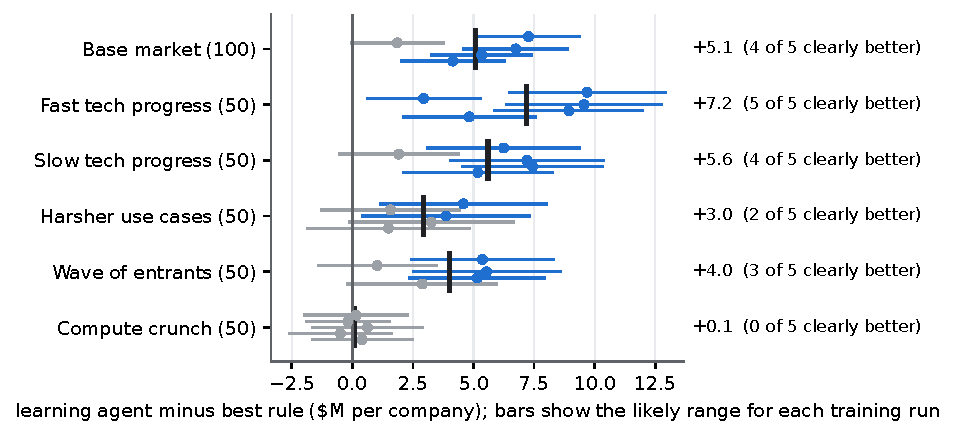
\includegraphics[width=\linewidth]{figures/fig_test.pdf}
\caption{Each agent's lead over the best rule, with its likely range (95\% confidence interval), in every test condition. Blue: clearly better; grey: not clearly different. Black bar: average of the five runs.}
\label{fig:test}
\end{figure}

\textbf{Normal markets.} Across 100 new markets the agents created \$19.3M per company on average against \$14.3M for the best rule, a lead of \$5.1M, with a likely range of \$2.6M to \$7.7M once both market and training-run luck are counted (Table~\ref{tab:test}). The lead varied between runs from \$1.9M to \$7.3M (standard deviation \$2.2M). Four agents were clearly better than the rule; the fifth led by \$1.9M with an interval that just reached zero ($-0.03$ to $+3.8$). Survival to month 120 was 97--100\% for the agents and 97\% for the rule. By our own pre-set bar the result is a narrow miss: the average lead clears \$3M comfortably, but only four of five agents were clearly better.

To read a \gl{confidence interval}: it is the range in which the true average lead most likely lies, given the luck of the particular markets tested; when the whole range is above zero we call the agent clearly better.

\textbf{How the intervals were calculated.} For one agent in one condition, each test market gives one paired difference: the agent's value created (the average of its three sampled plays, or its single greedy play) minus the rule's value in the same market. The three plays are averaged before differencing, so a market counts once. The pre-registered interval is the mean of these $n$ differences $\pm\,1.96\,s/\sqrt{n}$, where $s$ is their standard deviation (a normal approximation). As a check we also resampled markets with replacement 10{,}000 times (a percentile bootstrap); the two methods' interval ends agree within \$0.3M, every main agent's classification is the same under both, and the fifth agent remains just short of clearly better ($-0.02$ to $+3.8$). The five agents play the same test markets, and their leads move together from market to market (average correlation 0.7), so they are not five independent pieces of evidence. For the five-agent average we therefore resample both the training runs and the markets (a two-level bootstrap), which counts both kinds of luck; these are the ranges in Table~\ref{tab:test}. Full details and all intervals are in \texttt{results/v2/intervals.json}.

\textbf{Other conditions.} The agents' lead held when technology moved faster (all five clearly better) or slower (four of five) and with a wave of new entrants. With harder use cases the average lead was positive but its likely range included zero. In the compute crunch, where chip shortages are three times as likely and deeper and new capacity takes longer, there was \emph{no statistically detectable difference} between the agents and the rule (both \$5.3M; lead $+0.1$, likely range $-1.7$ to $+2.0$). That is not the same as equal performance: a difference of up to about \$2M either way is compatible with the data. The agents also survived less often (46--74\% against 80\%), so whatever they earned came with more risk.

\textbf{Testing many comparisons at once.} The success bar is a single primary endpoint, fixed in advance: five per-agent tests in normal markets. The other conditions are secondary, and looking at many comparisons raises the chance that one looks clear by luck. With a Holm correction for the family-wise error rate \citep{holm1979} across all 30 per-agent tests (five agents, six conditions), 15 of the 18 clear leads remain clear, including all four in normal markets. Across the six pooled five-agent tests, the leads in normal markets, faster and slower technology progress and the wave of entrants remain clear; harder use cases and the crunch remain unclear. The conclusions do not change.

\textbf{Practice scores flatter.} On the practice markets the kept versions led the rule by \$7.8M on average in normal markets; on the test markets the lead was \$5.1M, about \$2.8M less. Choosing the best of many versions by a noisy score picks versions that were partly lucky, so their score overstates how well they will do next time. This is why the test markets were kept untouched. The ordering was nonetheless informative: the runs with the highest and lowest practice scores (runs 5 and 4) also had the highest and lowest test results.

\textbf{How strong is the yardstick?} Best expected value is a hand-built rule, not a proven optimum, so we tested it against an \emph{oracle} version that is given every use case's true hidden difficulty, on 50 fresh markets (seeds 500--549). Perfect knowledge did not help it: the oracle created \$13.3M against the rule's \$14.3M in normal markets (difference $-1.0$, likely range $-4.1$ to $+2.4$) and \$6.1M against \$5.3M in the crunch ($+0.8$, range $-1.6$ to $+3.6$). The rule is therefore not held back by poor estimates of difficulty, and the agents' lead does not come from estimating difficulty better: on the same markets they beat the oracle by \$7.6M (range $+3.5$ to $+11.5$). It comes from something the rule does not model at all, which the switch-off tests below identify as competition. These fresh markets also replicate the main test: the agents led the rule by \$6.6M (range $+3.3$ to $+10.0$) in normal markets and by \$0.0M (range $-2.3$ to $+2.3$) in the crunch. The oracle is an information upper bound for this one rule, not for the game; we did not compute the best possible strategy, which is out of reach for a game of this size.

\subsection{What each change contributes}
\label{sec:controls}

\begin{figure}[h]
\centering
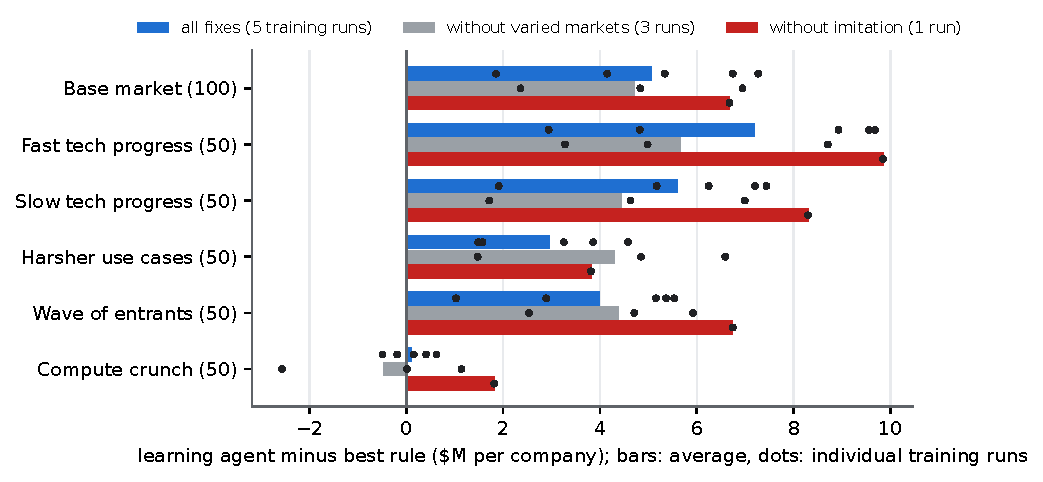
\includegraphics[width=\linewidth]{figures/fig_controls.pdf}
\caption{Lead over the best rule on the test markets for the full recipe and three comparison arms, five training runs each. Bars show averages; dots show individual runs. The two no-imitation runs at about $-14$ to $-16$ went bankrupt in every market.}
\label{fig:controls}
\end{figure}

To see which parts of the recipe matter, we compared three arms of five runs each, using the same training seeds as the full recipe so that each comparison is paired by run as well as by market (Figure~\ref{fig:controls}). For each arm we also report the smallest true difference from the full recipe that the comparison would detect with 80\% probability (its \gl{statistical power}), computed from the two-level bootstrap.

\begin{table}[h]
\centering
\footnotesize\setlength{\tabcolsep}{3pt}
\begin{tabular}{lrrrr}
\toprule
Arm (5 runs, normal markets) & Lead over rule & Minus full recipe & Detectable at 80\% power & Survival \\
\midrule
Full recipe & $+5.1$ ($+2.6$ to $+7.6$) & -- & -- & 98\% \\
No varied markets & $+5.0$ ($+2.7$ to $+7.4$) & $-0.1$ ($-2.4$ to $+2.3$) & \$3.4M & 98\% \\
No imitation & $-2.5$ ($-12.3$ to $+7.1$) & $-7.6$ ($-17.6$ to $+2.0$) & \$14.3M & 59\% \\
Imitation only, no RL & $+0.4$ ($-1.2$ to $+2.1$) & $-4.7$ ($-7.0$ to $-2.4$) & \$3.3M & 98\% \\
\bottomrule
\end{tabular}
\caption{The comparison arms on the 100 normal test markets (\$M per company, likely ranges from resampling runs and markets). The first two arms were run under the original plan and the revision plan; ``imitation only'' is each full-recipe run's network after imitation and before any reinforcement learning.}
\label{tab:arms}
\end{table}

\textbf{Training on varied markets brought no detectable benefit.} The five agents trained only on normal markets led the rule by \$5.0M, against \$5.1M for the full recipe (difference $-0.1$, likely range $-2.4$ to $+2.3$), and by $-0.4$ against $+0.1$ in the crunch (difference $-0.4$, range $-2.0$ to $+1.2$). With five runs each, a true difference of \$3.4M in normal markets (\$2.3M in the crunch) would have been detected four times out of five, so any benefit is smaller than that. One explanation is that the varied conditions stayed deliberately mild, short of the test conditions.

\textbf{Imitation makes training reliable.} Three of the five runs trained from scratch learned well, leading the rule by \$5.7M to \$7.4M, as well as the imitation-started agents. The other two never escaped the trap described in Section~\ref{sec:learn}: they learned to do almost nothing, their exploration fell to the floor and stayed there, and they went bankrupt in every test market. All five imitation-started runs succeeded. Learning from scratch can work with this recipe, but it is a gamble; imitation removes that risk.

\textbf{Reinforcement learning adds real value on top of imitation.} The network straight after imitation, before any reinforcement learning, behaved much like the rule it copied: a lead of \$0.4M (range $-1.2$ to $+2.1$), with no agent clearly better. Reinforcement learning then added \$4.7M (range $+2.4$ to $+7.0$), clearly above zero, and similar gains in every condition except the compute crunch. There, reinforcement learning added nothing ($+0.3$, range $-1.6$ to $+2.1$) and cut survival from 82\% for the imitation-only networks to 61\%: the extra risk the trained agents take pays in normal markets but not in a crunch.

\textbf{What remains.} All arms shared the other changes: the larger set of practice markets with greedy or sampled play, longer patience before early stopping, the exploration floor and the wider mix of rivals. These are the likely source of the reinforcement-learning gain, but we did not test them one at a time, so this remains a hypothesis.

\subsection{A new method: Paired-Fork Advantage against a Rule}
\label{sec:pfar}

The results so far point to one weakness of standard training: the agent's learning signal is weakest exactly where it matters. When it starts a project, the result appears 8--12 months later, mixed with everything else that happened meanwhile, and PPO must guess from its value function how much credit the decision deserves. Two of five runs learning from scratch never escaped doing nothing, plausibly for this reason. We therefore designed an estimator that uses a property most RL environments lack and economic simulators have: the market can be copied mid-game, future randomness included.

\textbf{The idea.} At a decision where the agent's action $a$ differs from the best-expected-value rule's action $b=\text{rule}(s)$, we copy the market twice. Copy A takes $a$, copy B takes $b$; every other company's action that month is the same. Both copies then run $H=12$ months with the current policy for all learning companies, a sampling generator seeded identically in both, and every random stream of the market shared (shocks, gate outcomes, entry, customer choices), a technique known as \gl{common random numbers}. The PFAR advantage is
\begin{equation}
A^{\text{PFAR}}(s,a) = \sum_{k=0}^{H-1} \gamma^k \frac{r^{A}_{k} - r^{B}_{k}}{\sigma} + \gamma^{H}\big(V(s^{A}_{H}) - V(s^{B}_{H})\big),
\end{equation}
with the training reward $r$, its running scale $\sigma$, the current value function $V$, and no value after bankruptcy. It replaces the usual advantage estimate for that sample; value targets are unchanged.

\textbf{Why it is a valid signal.} A policy-gradient update stays unbiased if the advantage subtracts any baseline that does not depend on the action taken \citep{sutton2018rl}. The second copy estimates the value of the rule's action, $Q(s,\text{rule}(s))$, which depends only on the state: the rule is deterministic. So $A^{\text{PFAR}}$ estimates $Q(s,a) - Q(s,\text{rule}(s))$, up to the truncation at $H$ months and the value estimate at the end. Because both copies see the same luck, the shocks and gate draws that make single returns so noisy largely cancel. It also reads naturally: the agent learns ``was my choice better than the expert's, here?'', which is exactly how it is evaluated.

\textbf{Budget and cost.} We fork a random share of disagreeing decisions, about four per market per update, so the fork probability is $\min(0.25,\,4/D)$ where $D$ is the number of disagreements in the previous update. A market copy takes about 7\,ms and a fork about 0.15--0.35\,s, so PFAR training ran at roughly a quarter to a half of the speed of plain PPO. Automated checks confirm that a copy given the same actions follows exactly the same history and that forking never changes the real game.

\textbf{Does shared luck reduce noise here?} Shared randomness does not always help \citep{sakib2026luck}, so we measured it directly, as planned in advance. On 185 decisions in markets 800--819 where the agent and the rule disagreed, we estimated the fork advantage eight times with the two copies sharing their randomness and eight times with independent randomness. Sharing cut the variance of the estimate by a factor of 1.7 overall and 3.9 for the typical decision, and reduced it for 79\% of decisions. This is the variance of the advantage signal, not of the whole update.

\begin{figure}[h]
\centering
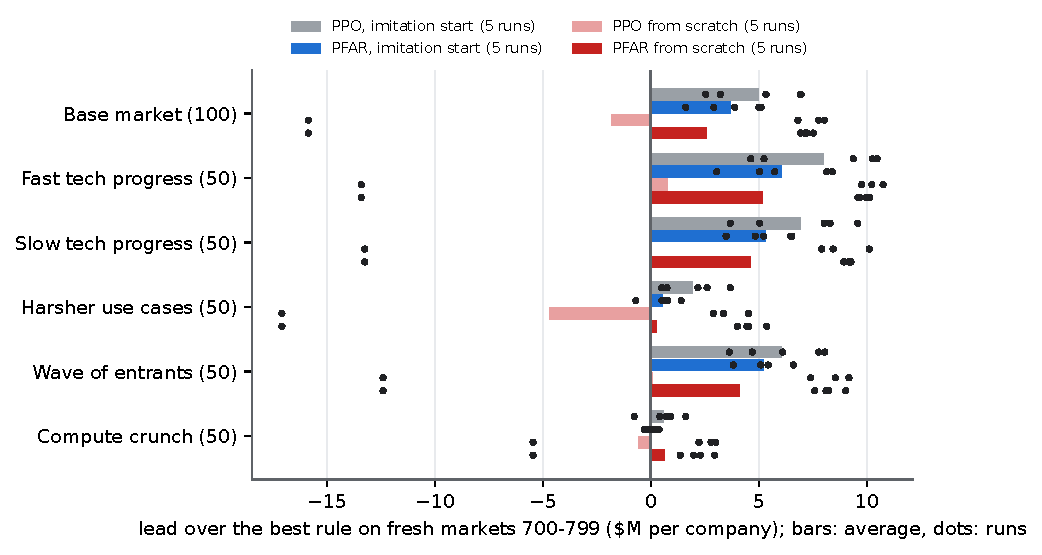
\includegraphics[width=\linewidth]{figures/fig_pfar.pdf}
\caption{PFAR against plain PPO on fresh markets 700--799 (normal) and 700--749 (other conditions), five runs per arm. Bars show averages; dots show individual runs. Runs near $-16$ learned to do nothing and went bankrupt in every market.}
\label{fig:pfar}
\end{figure}

\begin{table}[h]
\centering
\footnotesize\setlength{\tabcolsep}{4pt}
\begin{tabular}{lrrrr}
\toprule
Arm (5 runs) & Lead, normal markets & Clearly better & Lead, crunch & Survival, crunch \\
\midrule
PPO, imitation start & $+5.0$ & 5 of 5 & $+0.6$ & 51\% \\
PFAR, imitation start & $+3.7$ & 4 of 5 & $+0.0$ & 49\% \\
PPO from scratch & $-1.8$ & 3 of 5 & $-0.6$ & 34\% \\
PFAR from scratch & $+2.6$ & 4 of 5 & $+0.6$ & 44\% \\
\bottomrule
\end{tabular}
\caption{PFAR test on fresh markets (\$M per company over the best rule). Averages include runs that learned to do nothing.}
\label{tab:pfar}
\end{table}

\textbf{What the test showed.} We fixed three hypotheses before any PFAR run and tested every agent once on fresh markets (Figure~\ref{fig:pfar}, Table~\ref{tab:pfar}). \emph{P1, better agents:} not supported. Starting from imitation, PFAR led the rule by \$3.7M against \$5.0M for plain PPO; the difference, $-1.3$ (likely range $-3.6$ to $+0.9$), is not distinguishable from zero and points the wrong way. \emph{P2, better survival in the crunch:} not supported (49\% against 51\%, difference $-1.6$ points, range $-8$ to $+6$). \emph{P3, more reliable learning from scratch:} met by the pre-set bar of four successful runs out of five, against three for plain PPO, but this is a difference of one run, and the lead difference ($+4.4$, range $-9.4$ to $+18.0$) is far from clear. The same training seed (3) failed with and without PFAR; seed 4 failed with plain PPO and succeeded with PFAR.

\textbf{What we conclude.} PFAR produced a measurably cleaner learning signal, but on this evidence that did not translate into better agents, and its benefit for learning from scratch is at most suggestive. Two explanations seem plausible and are testable: only about 1--4\% of decisions were forked, so the cleaner signal touched few updates; and a 12-month horizon may still be short relative to the 8--12-month payoffs it is meant to capture. We report PFAR as a new, cheap-to-describe estimator with a pre-registered null result on performance, not as an improvement.

\textbf{A side result: imitation trades ceiling for reliability.} On these fresh markets, the runs that learned from scratch and succeeded led the rule by \$6.8M to \$8.0M, more than any imitation-started run (\$1.6M to \$6.9M). Imitation made training reliable (every imitation-started run succeeded) but appears to anchor the agent near the rule it copied. The fresh markets also replicate the main result: plain PPO from imitation led by \$5.0M with all five runs clearly better.

\subsection{One game, month by month}

\begin{figure}[h]
\centering
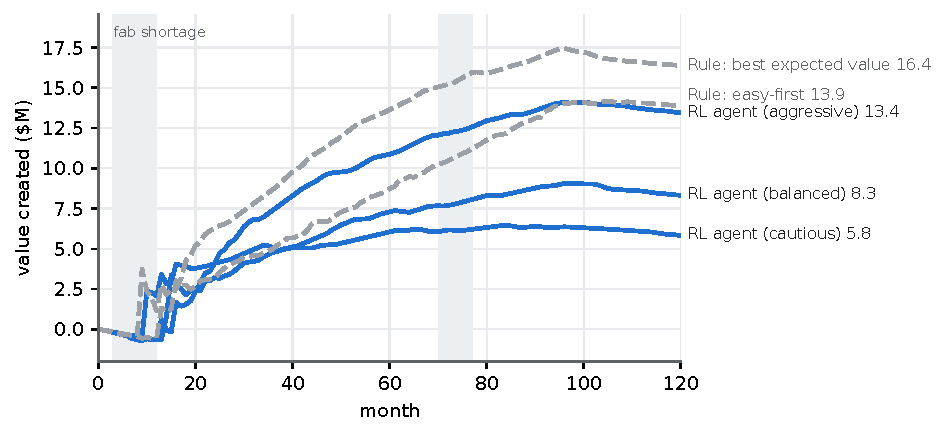
\includegraphics[width=\linewidth]{figures/fig_one_game.pdf}
\caption{One 120-month market (seed 47, chosen before the agents were trained) with three agent-run and two rule-based founding companies. Shaded: fab shortages.}
\label{fig:onegame}
\end{figure}

A single game shows how much luck matters (Figure~\ref{fig:onegame}). In this market the best-expected-value company finished highest (\$16.4M), followed by the easy-first company (\$13.9M) and the aggressive agent company (\$13.4M); the balanced and cautious agent companies earned \$8.3M and \$5.8M. Every founding company launched three products and survived, while four of eleven later entrants went bankrupt. Values flatten in the final years because only profit that can still be earned before the game ends is counted. One game proves little, which is why the test uses hundreds of markets.

\subsection{The strategy the learner discovered}
\label{sec:behaviour}

To see how the agent behaves among rivals of every kind, we ran run 1's agent in 30 separate analysis markets (seeds 200--229) with two agent companies, one company of each rule, and new entrants split between the agent and the best-expected-value rule (460 companies in all).

\begin{table}[h]
\centering
\small\setlength{\tabcolsep}{4pt}
\begin{tabular}{lrrrr}
\toprule
Behaviour (normal market, mixed rivals) & Agent & Best exp.\ value & Cash-pres. & Easy-first \\
\midrule
Value created per company & \$8.6M & \$2.4M & \$6.5M & \$2.6M \\
Survival at month 120 & 94\% & 64\% & 83\% & 63\% \\
True difficulty of use cases started & 0.61 & 0.52 & 0.48 & 0.39 \\
Starts in the regulated sector & 29\% & 15\% & 3\% & 30\% \\
Starts on the frontier model & 65\% & 44\% & 0\% & 100\% \\
Budget lean / standard / premium (\%) & 4/61/34 & 34/17/49 & 100/0/0 & 0/100/0 \\
Pilots refused (customers not ready) per company & 1.9 & 7.4 & 2.8 & 0.0 \\
Technical failures per company & 1.3 & 0.6 & 0.9 & 0.5 \\
Decisions spent scaling a product & 0\% & 1.5\% & 1.6\% & 2.6\% \\
\bottomrule
\end{tabular}
\caption{Behaviour of run 1's agent in 30 analysis markets with a mixed population of companies.}
\label{tab:behaviour}
\end{table}

Table~\ref{tab:behaviour} shows three patterns. First, the agent \emph{fails more and earns more}: it suffered twice the technical failures of the best-expected-value rule but aimed at harder, less crowded, more valuable use cases, including regulated ones the rule mostly avoided. The rule scores each use case in isolation; the agent learned that a use case many rivals are chasing is worth less than its spreadsheet value. Second, it learned \emph{timing}: the rule offered pilots to sectors not yet ready and was refused 7.4 times per company, while the agent mostly waited. Third, it \emph{never paid to scale up} a product, either a gap in what it learned or a sign that scaling is overpriced in this simulation. Among the agent's companies, risk appetite made little difference in normal markets (\$8.5M, \$8.9M and \$8.4M for cautious, balanced and aggressive).

\subsection{Which forces matter: switch-off tests}
\label{sec:ablation}

\begin{figure}[h]
\centering
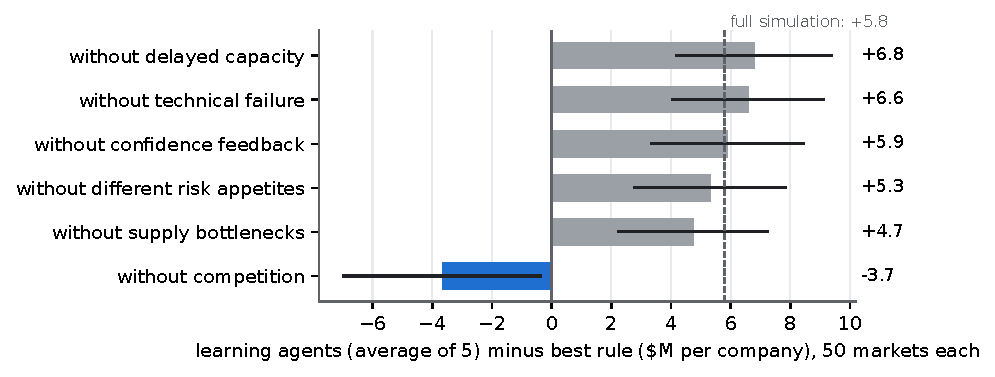
\includegraphics[width=\linewidth]{figures/fig_ablation.pdf}
\caption{Switch-off tests: the agents' lead over the best rule when one feature of the simulated market is turned off (50 markets each, average of the five agents). The dashed line marks the same comparison with every feature on.}
\label{fig:ablation}
\end{figure}

A \gl{switch-off test} (in the research literature, an ablation) turns off one part of a system and measures what changes. Keeping the trained agents unchanged, we turned off one market feature at a time (Figure~\ref{fig:ablation}). With every feature on, the agents led the rule by \$5.8M on these 50 markets. Turning off competition, so that each use case can be claimed by only one company, reversed the result: the rule earned \$14.0M against the agents' \$10.3M, a lead of $-$\$3.7M whose whole likely range lies below zero. The agents' habit of steering away from crowded use cases pays only when rivals exist; in a market without competition it leaves value on the table that the rule simply collects. Turning off any other feature (technical failure, confidence spreading between enterprises, supply bottlenecks, delays in building capacity, or differences in risk appetite) left the lead between $+$\$4.8M and $+$\$6.8M, within about \$1M of the full simulation and well within luck. Here each market's agent result is the average of the five agents, and the interval is over the 50 paired market differences. Within this model, then, the agents' edge comes from how they handle competition. A learned strategy is tuned to the world it trained in.

\subsection{How much the results depend on our numbers}
\label{sec:sensitivity}

\begin{table}[h]
\centering
\small
\begin{tabular}{lrrr}
\toprule
Parameter (normal value) & Changed to & Best rule & Agents' lead (likely range) \\
\midrule
None (normal market) & -- & \$14.3M & $+6.6$ ($+3.3$ to $+10.0$) \\
Price cut per rival (12\%) & 6\% & \$14.7M & $+7.4$ ($+4.3$ to $+10.6$) \\
 & 24\% & \$12.7M & $+6.6$ ($+3.4$ to $+10.1$) \\
Credit cost per month (1.2\%) & 0.6\% & \$14.1M & $+6.8$ ($+3.4$ to $+10.3$) \\
 & 2.4\% & \$14.2M & $+6.7$ ($+3.6$ to $+10.1$) \\
Price as share of customer value (32\%) & 24\% & \$10.4M & $+2.6$ ($-0.1$ to $+5.3$) \\
 & 40\% & \$16.7M & $+9.3$ ($+6.1$ to $+12.6$) \\
Overhead per month (\$25k) & \$15k & \$14.3M & $+7.1$ ($+4.1$ to $+10.3$) \\
 & \$40k & \$12.9M & $+7.2$ ($+3.7$ to $+10.8$) \\
\bottomrule
\end{tabular}
\caption{One parameter changed at a time, 50 fresh normal markets (seeds 500--549), the five agents unchanged. Ranges resample training runs and markets.}
\label{tab:sensitivity}
\end{table}

Every number in the simulation is an assumption, so we changed four of them, one at a time, to half and double (or similar) of their normal values, keeping the trained agents unchanged (Table~\ref{tab:sensitivity}). The agents stayed ahead of the rule in every case. The size of the lead hardly moved with competition's price cut, the cost of credit or overhead, but it tracked margins: when products can charge only 24\% of the value they create, the lead fell to \$2.6M and its range just reached zero; at 40\% it rose to \$9.3M. The qualitative finding is robust to these four choices; its size is not, and the agents were never trained at the changed values.

\subsection{How the market behaves}

The remaining results describe the simulated market itself, using the same 30 analysis markets.

\begin{figure}[h]
\centering
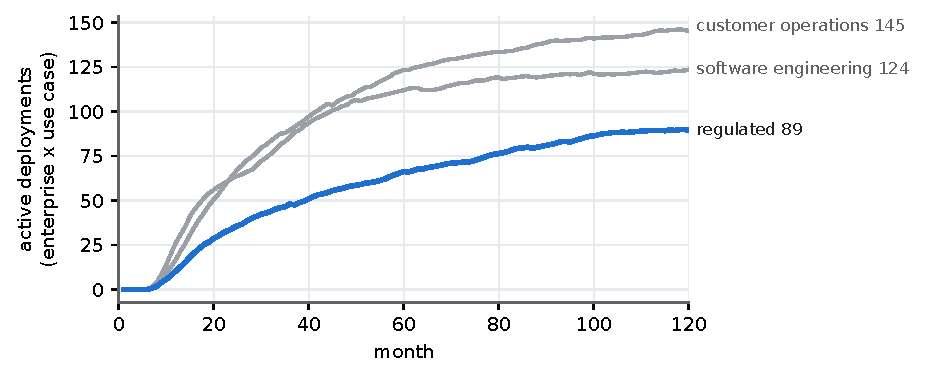
\includegraphics[width=\linewidth]{figures/fig_adoption.pdf}
\caption{Active deployments by sector, average of 30 normal markets. One deployment is one enterprise subscribed to one use case. Possible deployments per sector (enterprises with a need, summed over that sector's use cases) average 481, 413 and 384 for customer operations, software engineering and regulated industries.}
\label{fig:adoption}
\end{figure}

\begin{figure}[h]
\centering
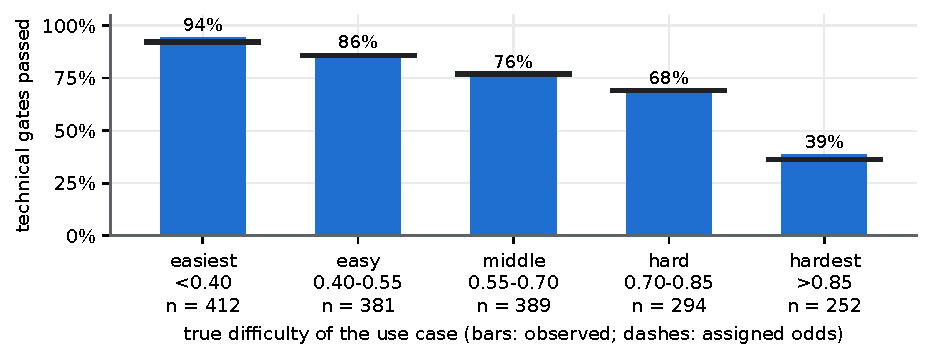
\includegraphics[width=\linewidth]{figures/fig_calibration.pdf}
\caption{Technical gate outcomes by true difficulty across 1,728 gates in 30 normal markets.}
\label{fig:calibration}
\end{figure}

Adoption follows S-curves in every sector (Figure~\ref{fig:adoption}), consistent with classic diffusion models \citep{bass1969diffusion}. We count adoption as \emph{deployments}: one enterprise subscribed to one use case. By month 120, customer operations has 125 active deployments (26\% of its 481 possible) and software engineering 115 (28\% of 413), but the regulated sector only 74 (19\% of 384) despite the largest budgets. Adoption levels off well below its potential because only use cases with a live product can be adopted, and budgets, value hurdles and each product's sales capacity limit the rest. The regulated sector's lag is about reliability, not demand: 23 of its 32 failed commercial gates failed on reliability, against none in the other two sectors.

Technical success fell from 94\% for the easiest use cases to 39\% for the hardest, within three points of the assigned odds in every band (Figure~\ref{fig:calibration}). In 247 cases where several companies launched the same use case (4.1 on average), the first launcher ended with 30\% of customers against an even share of 32\% (difference $-2.6$ points, likely range $-5.3$ to $+0.1$): no first-mover advantage when every company builds on the same models \citep{lieberman1988firstmover}. An earlier version of this analysis compared against one over the average number of launchers (24\%), which understates the fair share and wrongly suggested a modest advantage. Being early in the market did pay: founding companies created \$8.7M of value on average with 87\% survival, against \$3.8M and 74\% for the 310 later entrants.

\subsection{When the supply chain breaks}

In the compute-crunch condition, fab shortages are three times as likely, deeper (50--80\% of output) and longer (6--12 months), data centres start with 42\% less capacity, and new fab lines would take 24 months (in practice the fab never adds one).

\begin{figure}[h]
\centering
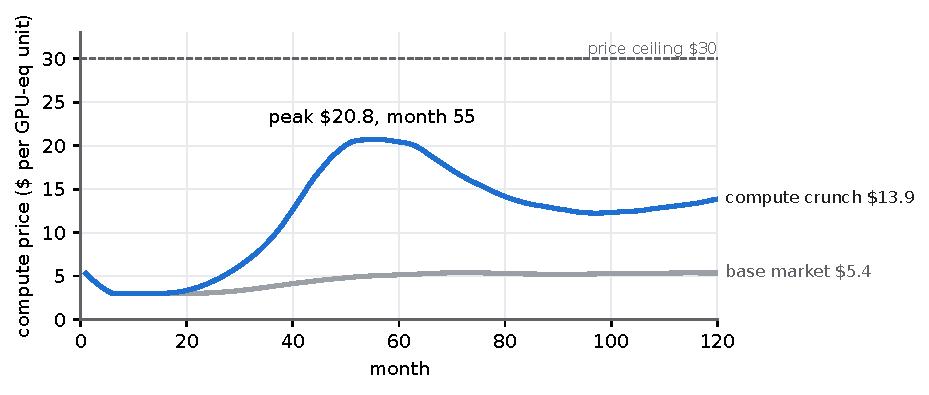
\includegraphics[width=\linewidth]{figures/fig_price.pdf}
\caption{Compute price, average of 30 markets per condition.}
\label{fig:price}
\end{figure}

\begin{figure}[h]
\centering
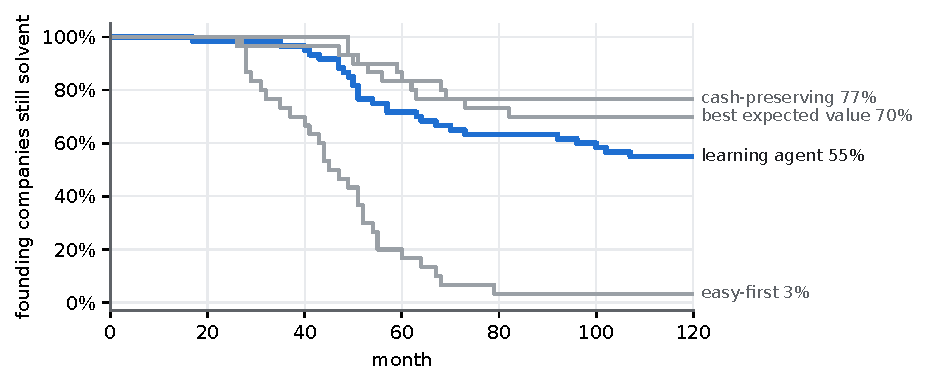
\includegraphics[width=\linewidth]{figures/fig_survival.pdf}
\caption{Share of founding companies still solvent in 30 compute-crunch markets with a mixed population.}
\label{fig:survival}
\end{figure}

Compute prices peak at 3.8 times the normal market's peak and end 2.6 times higher (Figure~\ref{fig:price}), because the shortages cut the chips available to data centres, which start smaller and take six months to install what they get, while the fab itself never expands: a delayed response reminiscent of supply-chain dynamics such as the bullwhip effect \citep{lee1997bullwhip,sterman1989misperceptions}. The share of compute demand actually served falls to 80\% by month 39, cancellations rise 37\%, bankruptcies rise two and a half times (8.3 against 3.4 per market), and total value created for enterprises, AI companies and suppliers falls 34\%, from \$733M to \$485M per market.

The agent's companies struggle here too (Figure~\ref{fig:survival}): 55\% of its founding companies survived, against 70\% for the best-expected-value rule and 77\% for the cash-preserving rule, which also earned the most in this mixed population (\$4.7M per company against \$1.0M for the agent and \$0.1M for best expected value). The agent kept running three projects at a time on standard and premium budgets, with 56\% of starts on the expensive frontier model. Unlike in normal markets, risk appetite mattered: cautious agent companies earned \$1.3M against \$0.8M for aggressive ones. A crunch rewards conserving cash, a lesson the agent had little chance to learn because its varied training conditions were milder than this.

\textbf{Why the agents go bankrupt more often.} Following each focal company month by month in 50 fresh crunch markets (seeds 500--549) shows how. The agents' companies that went bankrupt failed at a median of month 55, when compute prices peak, while the rule's failed at a median of month 80. The agents put 75\% of their projects on the expensive frontier model and 53\% on premium budgets, against 44\% and 29\% for the rule. In the first three years both spent about the same (\$47k against \$44k a month); the difference appears when the shortage raises the cost of serving customers on compute-hungry products: the agents' failing companies burned \$91k a month on average while alive, against \$59k for the rule's. The extra risk is a bet on costly inputs that a price spike turns ruinous. Training with a stronger bankruptcy penalty might trade some value for survival; we have not tested this.

\subsection{How robust are the market findings?}
\label{sec:robust}

\begin{table}[h]
\centering
\scriptsize\setlength{\tabcolsep}{3pt}
\begin{tabular}{p{3.6cm}>{\centering\arraybackslash}p{1.1cm}>{\centering\arraybackslash}p{1.3cm}>{\centering\arraybackslash}p{1.8cm}>{\centering\arraybackslash}p{1.4cm}>{\centering\arraybackslash}p{1.2cm}>{\centering\arraybackslash}p{1.3cm}}
\toprule
Changed parameter & Half adoption (month) & Regulated vs.\ others & First launcher / fair share & Founders vs.\ entrants & Crunch price peak & Crunch value change \\
\midrule
None (normal settings) & 26 & 0.59 & 30\% / 31\% & 2.1$\times$ & 3.9$\times$ & $-$35\% \\
Adoption steepness 2 (normal 4) & 27 & 0.56 & 30\% / 31\% & 2.1$\times$ & 4.0$\times$ & $-$35\% \\
Adoption steepness 8 & 26 & 0.59 & 33\% / 31\% & 2.5$\times$ & 3.8$\times$ & $-$34\% \\
Price cut per rival 6\% (12\%) & 24 & 0.57 & 30\% / 30\% & 2.1$\times$ & 3.7$\times$ & $-$32\% \\
Price cut per rival 24\% & 27 & 0.59 & 31\% / 31\% & 2.4$\times$ & 3.6$\times$ & $-$34\% \\
Entry rate 2\% (4\%) & 27 & 0.56 & 30\% / 32\% & 2.2$\times$ & 3.8$\times$ & $-$35\% \\
Entry rate 8\% & 26 & 0.62 & 28\% / 30\% & 2.3$\times$ & 4.0$\times$ & $-$33\% \\
Compute price ceiling \$15 (\$30) & 26 & 0.59 & 30\% / 31\% & 2.1$\times$ & 2.6$\times$ & $-$24\% \\
Compute price ceiling \$60 & 26 & 0.59 & 30\% / 31\% & 2.1$\times$ & 4.2$\times$ & $-$37\% \\
Confidence spreading 0.15 (0.3) & 25 & 0.57 & 31\% / 31\% & 2.4$\times$ & 4.0$\times$ & $-$34\% \\
Confidence spreading 0.6 & 26 & 0.59 & 30\% / 31\% & 2.1$\times$ & 3.9$\times$ & $-$36\% \\
Fab build time 12 months (18) & 26 & 0.59 & 30\% / 31\% & 2.1$\times$ & 3.9$\times$ & $-$35\% \\
Fab build time 24 months & 26 & 0.59 & 30\% / 31\% & 2.1$\times$ & 3.9$\times$ & $-$35\% \\
\bottomrule
\end{tabular}
\caption{The market findings with one structural parameter changed at a time, 30 fresh markets each (seeds 600--629), in the normal market and the compute crunch. ``Half adoption'' is the month by which half of the final deployments exist; the crunch columns compare each crunch variant with the matching normal variant.}
\label{tab:robust}
\end{table}

The market findings are consequences of parameters we chose, so we changed six structural parameters one at a time, to a low and a high value, and reran 30 fresh markets for each (Table~\ref{tab:robust}). Every qualitative finding kept its direction in every variant: adoption reached half its final level by month 24--27 with new deployments peaking around month 14; the regulated sector stayed at 56--62\% of the other sectors' deployments; the first launcher's share stayed within three points of a fair share (no first-mover advantage); founding companies created 2.1--2.5 times the value of later entrants; and a compute crunch raised the compute-price peak 3.6--4.2 times and cut total value created by 32--37\%. The one exception in size is the compute price ceiling: halving it shrank the crunch's price spike to 2.6 times and its value loss to 24\%. Two parameters had no effect at all, and we flag them rather than count them as robustness checks: the fab's build time, because the fab never expands in our markets, and the price ceiling in normal markets, which prices never reach.

\section{From simulated findings to real-world hypotheses}
\label{sec:lessons}

The experiments in Section~\ref{sec:results} establish consequences of the model's assumptions, not facts about actual AI markets. Reliability thresholds, competition rules, capacity delays, confidence dynamics and every price were chosen by us; the simulation shows what follows if they hold. We therefore state each possible real-world implication as a hypothesis, name the modelled assumptions it rests on, and say what evidence would test it (Table~\ref{tab:hypotheses}). Where a switch-off test turned a mechanism off (Section~\ref{sec:ablation}), we know that the finding depends on that mechanism within the model; for the others, the dependence is inferred from the model's structure. Two findings (H1 and H9) concern the learning method rather than the market, and their transfer to people and organisations is an analogy, not a result.

\begin{table}[!htbp]
\centering
\scriptsize
\renewcommand{\arraystretch}{1.25}
\begin{tabularx}{\linewidth}{>{\raggedright\arraybackslash}p{0.4cm}LLL}
\toprule
 & Simulated finding & Depends on these modelled assumptions & Evidence needed in real markets \\
\midrule
H1 & Learning from scratch succeeded in three of five runs despite payoffs arriving 8--12 months after spending; the other two learned to do nothing. Starting from imitation succeeded five times out of five. & Payoffs behind a fixed sequence of stages; a fairer score that counts work in progress as an asset. & Analogy only: whether organisations that protect early experimentation sustain more multi-stage innovation projects. \\
H2 & The agent accepted twice the technical failures for harder, less contested use cases and created 3.5$\times$ the value of the best rule among mixed rivals. & Success odds fall smoothly with difficulty; value is independent of difficulty; each rival cuts price 12\%. Switch-off test: the lead reverses without competition. & Project-level data linking difficulty, failure, competition and returns across AI deployments. \\
H3 & The regulated sector adopted slowest despite the largest budgets; 23 of 32 failed pilots failed on reliability. & An 84--92\% reliability floor applied as a hard pass/fail gate; model reliability rising about one point per release. & Adoption timing in regulated industries against the measured reliability of available models. \\
H4 & Pilots offered to unready sectors were refused 7.4 times per company (1.9 for the agent). & Confidence is shared and spreads within a sector and scales adoption. Switch-off test: removing it barely changes the agents' lead. & Whether one vendor's failure measurably lowers other vendors' pilot acceptance in the same sector. \\
H5 & A fab shortage raised compute prices 3.8$\times$ and they stayed 2.6$\times$ higher; value created fell 34\%. & Shortage frequency and depth chosen by us; slow data-centre installation; a bounded price rule driven by utilisation; a fab that never expands. Robustness: the spike shrinks to 2.6$\times$ with a lower price ceiling. & Compute price and availability around real capacity shocks; downstream failure rates. \\
H6 & The first launcher kept 30\% of customers against a 32\% even share; founding companies earned 2.3$\times$ later entrants. & All companies access the same models; customers compare offers on value; a finite set of use cases. & Market share by launch order for comparable products built on shared foundation models. \\
H7 & Agents led the best rule in five of six market conditions (clearly in four), but showed no detectable difference from it in a supply crunch while going bankrupt more often; risk appetite mattered only in the crunch. & Condition parameters we specified; agents trained on milder varied conditions. & Strategy performance across real periods of abundant and scarce compute. \\
H8 & Without competition, the best rule beat the agents by \$3.7M, reversing their \$5.8M lead. & Competition modelled as price discounts and customer choice. & As H2, plus whether selection rules that ignore rivals underperform in crowded markets. \\
H9 & Practice-market scores overstated test performance by about \$2.8M; the agents' lead varied from \$1.9M to \$7.3M between identical training runs. & Variance of this simulator, the training procedure and the selection of the best version. & Methodological; consistent with RL evaluation practice \citep{henderson2018matters,agarwal2021precipice}. Transfer to choosing among business pilots is an analogy. \\
H10 & Agents that learned from scratch and succeeded beat imitation-started agents (\$6.8M--\$8.0M against \$1.6M--\$6.9M), but two of five failed outright. & The imitation target was a single rule; fixed training budget. & Analogy only: whether copying established practice limits later improvement while making it safer. \\
\bottomrule
\end{tabularx}
\caption{Each simulated finding, the assumptions it rests on, and the evidence a real-world claim would require.}
\label{tab:hypotheses}
\end{table}

\textbf{From model numbers to real quantities.} No parameter was estimated from data. Table~\ref{tab:params} lists the parameters the hypotheses lean on most, what each stands for, and what we know about how much it matters here. Where a hypothesis rests on an untested parameter (H3, H5), only its direction should be carried over, and only as a question for data.

\begin{table}[h]
\centering
\scriptsize
\renewcommand{\arraystretch}{1.2}
\begin{tabularx}{\linewidth}{>{\raggedright\arraybackslash}p{3.0cm}lLL}
\toprule
Parameter & Value & Real-world counterpart & What we know about its influence here \\
\midrule
Price cut per rival & 12\% & discounting as competitors enter one use case & Agents' lead holds from 6\% to 24\% (Table~\ref{tab:sensitivity}); without competition it reverses (H2, H8). \\
Price as share of customer value & 32\% & how much of the value created a vendor can capture & Lead shrinks to borderline at 24\%, grows at 40\%. \\
Credit cost & 1.2\%/month & cost of debt for young companies & Lead unchanged from 0.6\% to 2.4\%. \\
Reliability needed, regulated sector & 84--92\% & compliance thresholds for AI in regulated work & Not varied; H3's size depends directly on it. \\
Fab shortage odds and depth & 2\%/month, 30--60\% (crunch 6\%, 50--80\%) & frequency and severity of chip supply shocks & Not varied beyond the two conditions; H5's size depends directly on them, and on the compute price ceiling (Section~\ref{sec:robust}). \\
Capacity lead times & 18--24 months fab, 3--6 months install & time to add real fabrication and data-centre capacity & Fab build time has no effect: the fab never invests in our markets. Install time not varied. \\
\bottomrule
\end{tabularx}
\caption{Key parameters behind the hypotheses. Values are illustrative, chosen to be plausible, not measured.}
\label{tab:params}
\end{table}

Read this way, the findings are best treated as a map of where to look. The most robust within the model are those confirmed by a switch-off test, by many test markets or by repetition across training runs (H2, H7, H8, H9). The most assumption-bound are those whose size follows directly from parameters we chose (H3, H5). Where a mechanism has a documented real-world counterpart, the direction agrees with prior work, for example amplified supply-chain responses \citep{lee1997bullwhip,sterman1989misperceptions} and S-shaped diffusion \citep{bass1969diffusion}; the sizes have not been calibrated against data and should not be quoted as forecasts.

\section{Limitations}
\label{sec:limitations}

Every parameter is an illustrative choice rather than an estimate from data, and the model has not been calibrated or validated against real markets, so sizes of effects mean nothing outside the model; directions are more trustworthy, especially where a switch-off test isolates the mechanism. Five training runs per arm give only a rough picture of how much results vary between runs; differences below about \$3M between arms could go undetected, and we did not test the shared changes one at a time. The test covered six conditions without adjusting for multiple comparisons. A scoring error, found after the test, was corrected and the test games were replayed once (Appendix~\ref{app:audit}); training itself used the original scoring. Most agents were initialised by imitating the best-expected-value rule, so some of their behaviour may be inherited. Rankings depend on the rivals present: best expected value led cash-preserving in the test, with rule-based rivals, but trailed it with mixed rivals, and no result here is an equilibrium. The agents were trained on a risk-adjusted, discounted reward while we report undiscounted value (Appendix~\ref{app:reward}). Prices are a fixed share of value, enterprises do not switch providers mid-contract, upstream firms are scripted and always solvent, and model providers do not act strategically. PFAR forked only 1--4\% of decisions with a 12-month horizon; we did not test larger budgets or longer horizons, which are the obvious next step. Finally, the agent never chose to scale a product, which we cannot attribute to a learning gap or to the parameter choice.

\section{Conclusion}

A transparent simulation of the AI value chain reproduces recognisable dynamics: S-shaped adoption, reliability-gated regulated markets, sticky supply shocks and no lasting first-mover advantage. Reinforcement learning on a laptop produced agents that, on markets never seen before, created about a third more value than the strongest hand-written rule in normal conditions and led in most changed conditions, mainly by avoiding crowded opportunities and timing customer engagement. In a severe compute crunch there was no statistically detectable difference from the rule, and the agents went bankrupt more often. Writing the test plan down in advance kept us honest: the result narrowly missed our own bar, practice scores overstated real performance, training on varied markets brought no detectable benefit, reinforcement learning added a clear \$4.7M over imitation alone, and imitation turned learning from a gamble (three successes in five) into a reliable process (five in five). A new estimator, PFAR, which compares the agent's action with the expert's in two copies of the market sharing the same luck, gave a cleaner learning signal but, under a pre-registered test, no better agents. We hope the simulator serves both as a teaching tool for reinforcement learning and as a sandbox for generating hypotheses about AI markets that real data must then test.

\section*{Code and data availability}
{\sloppy The simulator, trained agents, evaluation data, figure scripts, the test plan written before the v2 experiments (\texttt{paper/PROTOCOL\_v2.md}; see Appendix~\ref{app:audit}) and a live viewer in which agents play without human input are available at \url{https://github.com/ravikadam/ai-economy-lab}. Built with PyTorch \citep{paszke2019pytorch}, with Gymnasium and PettingZoo adapters \citep{towers2024gymnasium,terry2021pettingzoo}.\par}

\section*{Acknowledgements}
\ifaixiv
This paper, the simulator code and the experiments were written and run by Claude Code (Anthropic), an AI system, working from an idea and continuing direction by Ravi Kadam, who set the goals, chose which reviews to answer and how, and reviewed the results. As corresponding human, Ravi Kadam takes responsibility for the submission.
\else
The simulator code, experiments and drafting of this paper were carried out with substantial assistance from Claude (Anthropic), an AI system. The author designed the study, directed the work, and reviewed the results and text, and takes full responsibility for the content.
\fi

\bibliographystyle{plainnat}
\bibliography{references}

\appendix
\section{Glossary}
\label{app:glossary}

\begin{description}[style=unboxed, leftmargin=0pt, itemsep=3pt]
\small
\item[Action.] One choice an agent makes in a month, such as starting a project or launching a product.
\item[Action mask.] A filter that removes impossible actions before the agent chooses, so it never wastes a decision on them.
\item[Advantage.] How much better an action turned out than the value function expected. Positive advantage makes the action more likely in future.
\item[Agent.] The decision-maker that learns; here, the software running one AI product company.
\item[Common random numbers.] Running two alternatives with exactly the same random draws, so that differences between them come from the alternatives rather than from luck.
\item[Confidence interval (95\%).] The range in which the true average most likely lies, given the luck of the markets tested. If the whole range is above zero, we call a lead clear.
\item[Credit-assignment problem.] Working out which earlier decisions deserve credit or blame for a reward that arrives much later.
\item[Domain randomisation.] Training on many randomly varied versions of the environment so that the agent does not depend on one set of conditions. We call it training on varied markets.
\item[Early stopping.] Ending training once the score on practice markets stops improving, and keeping the best version seen.
\item[Environment.] The world the agent acts in; here, the simulated AI economy.
\item[Episode.] One complete game from start to finish; here, 120 simulated months of one market.
\item[Bootstrap.] Estimating uncertainty by recomputing a result many times on data resampled with replacement, here test markets and training runs.
\item[Exploration.] Trying actions other than the one currently believed best, in order to discover better ones. Measured by the policy's entropy: higher means more varied choices.
\item[Exploration floor.] Our rule that raises the bonus for exploring whenever the agent's exploration falls below a set level.
\item[Imitation learning.] Training a network to copy an expert's recorded decisions (also called behaviour cloning). Here the expert was the best-expected-value rule.
\item[Observation.] What the agent can see when it decides: its finances, projects, a shortlist of use cases with noisy estimates, and last month's market data.
\item[Overfitting.] Becoming good at the specific situations seen in training but worse at new ones.
\item[Policy.] The agent's decision rule: a neural network that gives a probability for each possible action.
\item[Practice markets.] Markets used only to choose which version of the agent to keep, never for training or for the final test (also called a validation or development set).
\item[Pre-registration.] Writing down the test plan and the bar for success before seeing any results, so they cannot be adjusted afterwards. It is strongest when the plan is lodged with an independent, time-stamped registry.
\item[Proximal Policy Optimisation (PPO).] The learning method used here; it improves the policy in small steps, limiting how far it may change in one update.
\item[Reward.] The score the agent receives after each action; here, the monthly change in its company's value.
\item[Reward shaping.] Adding terms to the reward to make learning easier. Some forms only move credit earlier without changing the best strategy; ours also adds deliberate risk penalties (Appendix~\ref{app:reward}).
\item[Seed.] A number that fixes all the randomness of a market or a training run, so that it can be repeated exactly.
\item[Statistical power.] The chance that a comparison detects a true difference of a given size; here we report the difference it would detect four times out of five.
\item[Switch-off test.] Turning off one feature of the simulated market and measuring what changes (an ablation in the research literature).
\item[Value function.] The network's prediction of how much future reward to expect from the current situation.
\end{description}

\section{Reproducibility}

All results run on one laptop. Training and imitation markets use seeds of 1{,}000{,}000 and above (each training run shifts them by 10{,}000{,}000 times its run number); practice markets are seeds 1000--1019 (normal) and 2000--2019 (varied conditions); analysis markets are 200--229; test markets are 400--499. No test market was used before the test. Every parameter lives in YAML files under \texttt{config/}; the training recipe is \texttt{config/train\_v2.yaml}, and the comparison runs use \texttt{config/train\_v2\_nodr.yaml} and \texttt{config/train\_v2\_pure.yaml}.

\begin{table}[h]
\centering
\small
\begin{tabularx}{\linewidth}{lL}
\toprule
Step & Command (approximate time on an Apple M2 Pro) \\
\midrule
Automated checks & \texttt{pytest} (4\,s) \\
Train one agent & \texttt{python -m training.train --config config/train\_v2.yaml --seed 0} (13--30\,min) \\
Test (replay) & \texttt{python -m scripts.test\_v2 --runs "runs/v2-seed*" "runs/v2nodr-seed*" "runs/v2pure-seed*"} (8\,min) \\
Switch-off tests & \texttt{python -m scripts.ablate\_v2 --runs "runs/v2-seed*"} (6\,min) \\
Confidence intervals & \texttt{python -m scripts.ci\_v2} ($<$1\,min) \\
Imitation-only baseline & \texttt{python -m scripts.make\_bc\_baseline} (5\,min) \\
Yardstick, sensitivity, crunch & \texttt{python -m scripts.review\_r1} (17\,min) \\
Behaviour and market analysis & \texttt{python -m scripts.experiments --checkpoint results/v2/seed0/best.pt --seeds 200:229 --out runs/paper\_v2}; \texttt{PAPER\_DIR=runs/paper\_v2 python scripts/paper\_stats.py} \\
Figures & \texttt{python paper/make\_figures.py} \\
Live viewer & \texttt{streamlit run viewer/app.py} \\
\bottomrule
\end{tabularx}
\end{table}

Key settings: 120 months; 5 initial companies, at most 12, entry from month 12; 300 enterprises; 60 use cases, 24 visible at start; \$1.5M capital and \$400k credit per company; 3 projects per company; 12 candidate use cases per observation. PPO: learning rate $10^{-4}$ after imitation, clip 0.2, 4 epochs, minibatch 4{,}096, starting exploration bonus 0.01 (raised up to 0.05 when exploration falls below 0.25), GAE $\lambda=0.95$, discount 0.99 per month, 24 markets $\times$ 60-month stretches; practice check every 20 updates, early stop after 8 checks without improvement, at most 1{,}000{,}000 firm-months.


\section{Score, training reward and terminal handling}
\label{app:reward}

\textbf{Company value.} For company $f$ at the end of month $t$ (of $T=120$), with $m_t = T - t$ months remaining,
\begin{equation}
V_t = C_t - D_t + \sum_{j\in\text{live}} \max(0,\bar\pi_j)\,a(\min(24,m_t)) + \sum_{k\in\text{dev}} I_k\, w(\text{stage}_k)\,\min\!\big(1,\tfrac{m_t}{12}\big),
\end{equation}
where $C_t$ is cash, $D_t$ debt, $\bar\pi_j$ a live product's trailing monthly profit, $a(n)=\sum_{i=1}^{n}1.01^{-i}$ an annuity factor at 1\% a month, $I_k$ the money invested in a project still in development and $w$ a stage weight (0.6 in research and prototype, 0.8 when ready to pilot or piloting, 0.9 after a passed pilot, 0.3 after a failed gate; times 0.8 when paused). Abandoned projects are written off. At $t=T$ both sums are zero, so $V_T = C_T - D_T$. A bankrupt company's cash is liquidated and its projects count for nothing, so from bankruptcy on $V_t = -D_t$.

\textbf{Score.} The reported score (``value created'') and the raw reward are $r_t = (V_t - V_{t-1})/\$1\text{M}$. Over a whole game the sum telescopes: $\sum_{t=1}^{T} r_t = (V_T - V_0)/\$1\text{M}$, the change in cash minus debt from the start (\$1.5M of cash, no debt) to the end, or to bankruptcy. The book value of projects in development therefore moves credit earlier without changing this undiscounted total.

\textbf{Training reward.} PPO maximised the discounted sum of a risk-adjusted reward,
\begin{multline}
\tilde r_t = r_t - \delta\max(0,-r_t) - 0.02\,\beta\max\!\Big(0, 1 - \tfrac{\text{runway}_t}{\rho}\Big) - 0.01\,\tfrac{D_t}{\$400\text{k}} \\
 - 2\beta\,\mathbb{1}[\text{bankrupt at } t] - 0.01\,(\text{illegal actions}),
\end{multline}
with discount $\gamma=0.99$ per month, where $\delta$, $\beta$ and $\rho$ are the company's downside aversion, bankruptcy aversion and runway target (cautious 0.6, 3.0, 12 months; balanced 0.3, 1.5, 8; aggressive 0.1, 0.7, 4), and runway is months of cash plus unused credit at the current burn, capped at 36. The cash-stress terms apply only to companies still solvent. Rewards were divided by a running estimate of their scale before each update.

\textbf{What this does and does not preserve.} Potential-based shaping leaves the best strategy unchanged when the shaping term has the form $\gamma\Phi(s_{t+1})-\Phi(s_t)$ \citep{ng1999shaping}. Our book-value term enters as $\Phi(s_{t+1})-\Phi(s_t)$, without the factor $\gamma$, so under discounting it slightly rewards holding book value; and the risk terms in $\tilde r_t$ deliberately change the goal. The agent therefore optimises a discounted, risk-adjusted objective, while we report the undiscounted score $\sum_t r_t$. We make no claim that the two have the same best strategy.

\textbf{Terminal handling.} A game ends after month 120; a company's own episode ends earlier if it goes bankrupt, with no value bootstrapped after either end. Training rollouts are cut every 60 months, and the value function estimates what follows each cut. Advantages use generalised advantage estimation with $\lambda=0.95$.

\section{Audit trail for the test plan}
\label{app:audit}

\textbf{What the record shows.} The protocol (\texttt{paper/PROTOCOL\_v2.md}) and the training configuration were first committed to the public repository in commit \texttt{68bf412} (19 October 2026, 10:29 IST), together with the results. The repository therefore cannot independently prove when the protocol was written. The file system records the protocol as created at 01:19:37 IST, before the first training run's folder was created at 01:20:49, and last modified at 01:29:13, when the comparison-run addendum was added. The test began at 10:11. These local timestamps are consistent with the stated order but are not independent evidence; a public registry with its own timestamps would have been. We describe the plan as a protocol fixed before the v2 experiments, informed by an earlier exploratory study.

\textbf{Departures from the plan.}
\begin{itemize}
  \item The two comparison runs were added after training began (seed 0 was training) but before any test result existed.
  \item \emph{Scoring correction.} After the test, while checking the reward definition, we found that a bankrupt company's final value still counted its unfinished projects and recently live products (on average \$0.2M per bankruptcy, at most \$1.9M, in 60 rule-only check markets). We corrected the scoring so that a bankrupt company is worth $-D_t$, and replayed the same test games once. The agents' decisions do not depend on this value (it never enters what they observe), so every game played out identically: survival was unchanged for every agent in every condition, and only games containing a bankruptcy changed score, always downwards. The five-agent lead moved by at most \$0.1M in every condition, and no agent changed between clearly better and not clearly different; one comparison run (no imitation, harder use cases) did. The switch-off tests and the analysis markets were re-scored in the same way. Results before the correction are kept in \texttt{results/v2/*\_before\_scoring\_fix.json}. Training and the practice-market scores used the original scoring.
  \item \emph{Revision plan R1.} The analyses requested in review (two more runs without varied markets, four more without imitation, the imitation-only baseline, the oracle, the sensitivity checks and the crunch diagnostics) were written into the protocol and pushed to the public repository as commit \texttt{07c23fb} (22 October 2026, 04:29 IST) before any of them was run, giving this round an independent timestamp. The new arms were tested on the original test markets, which had already been used once; no agent or setting was tuned on them, and the original agents reproduced their earlier results exactly. The yardstick, sensitivity and crunch analyses used fresh markets 500--549.
  \item \emph{Revision plans R2 and R3.} The second-review analyses (commit \texttt{5cdc737}) and the PFAR method, arms, test and hypotheses (commit \texttt{577b583}), with one amendment capping the fork rate after a smoke test (commit \texttt{cc307cf}), were pushed before the corresponding runs. PFAR agents and the plain PPO agents they are compared with were tested once, together, on fresh markets 700--799.
  \item \emph{Intervals.} The bootstrap intervals, including the two-level interval for the five-agent average, were added after the test in response to review; the pre-registered per-agent interval is unchanged and decides the success bar.
\end{itemize}

\end{document}
